\documentclass[a4paper, 12pt]{article}

%\usepackage{natbib}
\usepackage[english]{babel}
\usepackage{amsmath, amssymb}
\usepackage{parskip}
\usepackage{graphicx}

\DeclareMathOperator*{\argmax}{argmax}

\begin{document}

\title{AA2 Practical Assignment}
\author{Maarten de Jonge, Koen Keune, Edwin Odijk,\\ Francesco Stablum, Marysia Winkels}
\maketitle

\section*{Introduction}
%something something sampling based fitted Q-iteration/value-iteration, something something continuous
This report describes the extension on an old AA1 assignment for the AA2 course. The existing predator/prey game's environment was changed from discrete to continuous, and the game was optimized using sampling based fitted Q-iteration/value-iteration.%\cite{ng_lecture}\cite{musze}

FVI (Fitted Value Iteration) is an algorithm that is suited for
continuous state spaces with continuos features extracted from
the state. 
The value function of a certain state is inferred by
extracting at first the features $\phi(s^{(i)})$ 
after having sampled some states 
$s^{(1)}\ldots s^{(i)} \ldots s^{(m)}$, 
and then by fitting via linear regression
the respective estimated state values $y^{(i)}$ 
in order to obtain the vector
of weights $\theta$.

The estimated state values $y^{(i)}$ are calculated as follows:
for each action $a$ and state $s^{(i)}$, 
$k$ state transitions are performed by using probabilities from 
an MDP model.
An estimated $Q$-value for the $\langle a,s^{(i)}\rangle$ pair is obtained
by averaging the sums of rewards of $s^{(i)}$ and
discounted value of the
state obtained from the transition from $s^{(i)}$.
In this step the $V$-function from the previous iteration has been used,
which, at the first iteration, has been set to 0.

These estimated $Q$-values are then used in a Bellman-like 
backup operator which selects the highest $Q$-value across all actions,
and for the specific current $s^{(i)}$.
This will become the current estimated $V$-value for $s^{(i)}$. 
This value is denoted
by the symbol $y^{(i)}$ in order to highlight the fact that it's 
a quantity that is subject to regression.

Once all $y^{(\cdot)}$ values have been obtained,
the previosly mentioned regression is performed.
This whole procedure is performed iteratively for a pre-determined
number of iterations.

\section*{Implementation} 
The algorithm has been implemented in one function
that resembles to a certain extent the pseudo-code
from Ng's lecture notes FIXME:ref.

Behavior has been parametrized by adding a number of lambda functions
as parameters to the function \texttt{fvi}:

\begin{itemize}
\item \texttt{sample\_states} is a function that returns the $s^{(1)}\ldots s^{(m)}$ sampled states
\item \texttt{sample\_actions} is a function that returns a set of sampled actions, which might be in principle sampled from a continuous distribution as well.
These action will then be used in order to calculate all $Q$-value
estimations for a certain state $s^{(i)}$.
\item \texttt{phi} is a function that will return a feature vector
$\phi(s^{(i)})$ for the state $s^{(i)}$ given as input.
A good feature vector representation is
crucial in order to obtain an acceptable regression.
\end{itemize}

The biggest change with regards to the discrete world previously implemented is
the action selection function. Rather than simply maximizing the value over a
small, finite set of actions, it now has to be maximized over an infinite
2-dimensional interval. Luckily, the value function is conveniently convex
(\ref{fig:V}) and can be optimized by means of gradient ascent or similar
methods.

\begin{figure}[h!]
  \centering
  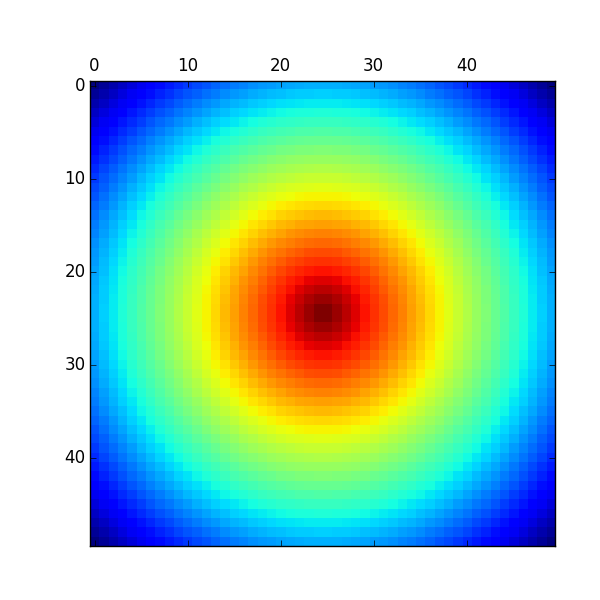
\includegraphics[width=0.5\textwidth]{V.png}
  \caption{A visual heatmap representation of the value function}
  \label{fig:V}
\end{figure}


We opted for a more brute-force method that makes use of the fact that
the $x$ and $y$ directions can be optimized seperately: Given a state $s$, first
the optimal action in the $x$ direction is calculated as
\[
  x' = \argmax_x V(transition(s, [x, 0]))
\]
followed by the optimal action in the $y$ direction:
\[
  y' = \argmax_y V(transition(s, [x', y]))
\]

\section*{Comparison of Algorithms}
%new implementations vs old results
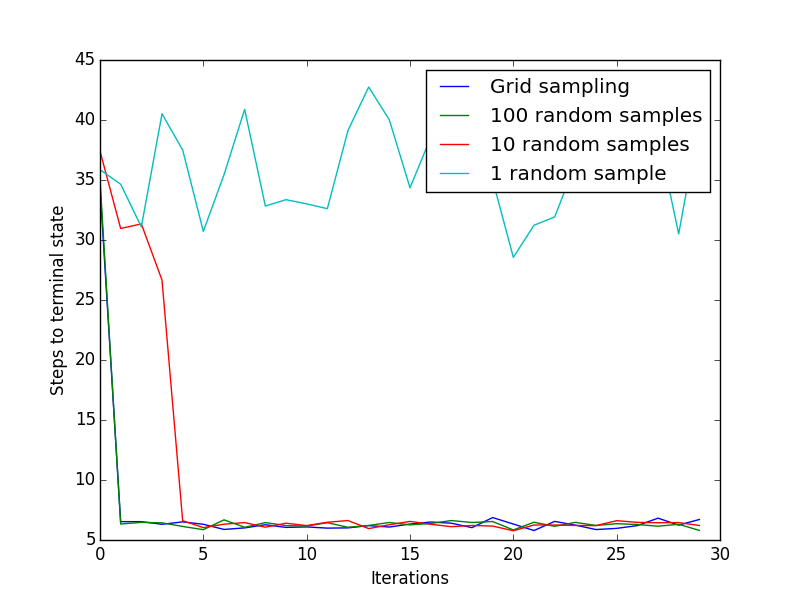
\includegraphics[scale=0.7]{convergence.png}
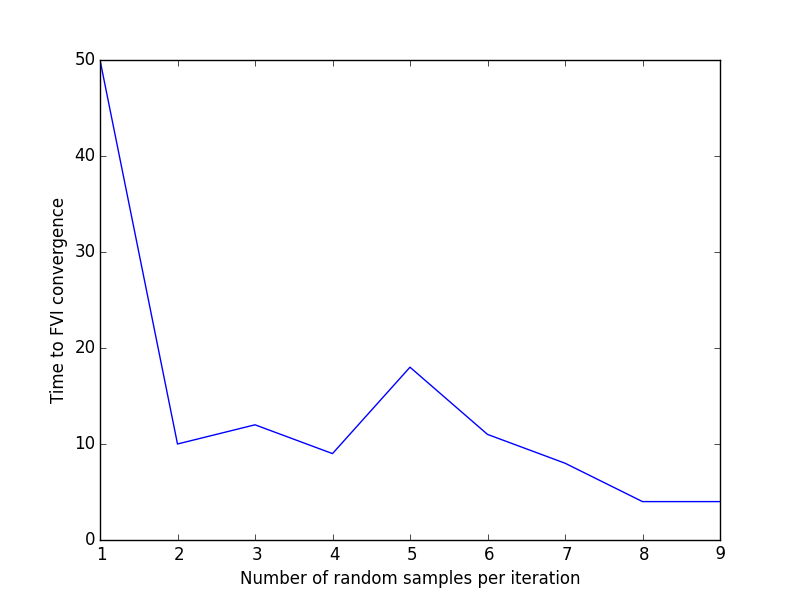
\includegraphics[scale=0.7]{n_samples.png}

\section*{Conclusion}
% ._.

\section*{References}
%\bibliographystyle{plain}
%\bibliography{ref}

\end{document}
